\section{BIP39: 从助记词生成确定性密钥}

BIP39提出了一种从助记词(Mnemonic Code)派生HD钱包种子的方法,
使得用户只需要掌握这组助记词即可借助钱包实现派生出HD钱包的密钥树,从而优化用户的交互体验.  
该协议主要包含两个过程: 从熵值(Entropy)生成助记词的过程以及从助记词派生种子的过程.
其中,助记词是从事先定义好的单词列表(Wordlist)里选出的符合相应长度要求的单词集合,
目前针对英语, 日语, 韩语, 西班牙语, 中文(简体/繁体), 法语, 意大利语都有相应的单词列表,
在使用前都对它们进行UTF-8编码处理,详见单词列表\footnote{
Wordlists. \url{https://github.com/bitcoin/bips/blob/master/bip-0039/bip-0039-wordlists.md}}.

用来产生助记词的熵值的比特长度为128到512比特,要求长度必须是32比特的整数倍.
熵值的比特长度越大,安全性就越高,但同时生成助记词中单词的个数也越多.
助记词的产生过程: 假设初始的熵值为$e$, 比特长度为$\textsf{bits}(e)$,
取$\textsf{SHA256}(e)$的前$\textsf{bits}(e)/32$比特作为检验和(Checksum)缀在$e$的后面,
随后将级联后的比特串以11比特为单位进行分组,即每个分组的数字范围是为$[0,\cdots,2047]$,
将其作为索引从单词列表中读取相应的单词,最终选出的词语即构成了一个助记词句子(Mnemonic Sentence).
当$\textsf{bits}(e)=128,192,256$时,对应的助记词的个数为12, 18, 24.
参见Figure~\ref{fig-entropy2mnemonic}(截取自``Mastering Bitcoin 2nd Edition - 
Programming the Open Blockchain''\footnote{
\url{https://github.com/bitcoinbook/bitcoinbook}}).

\begin{figure}[h]
\centering
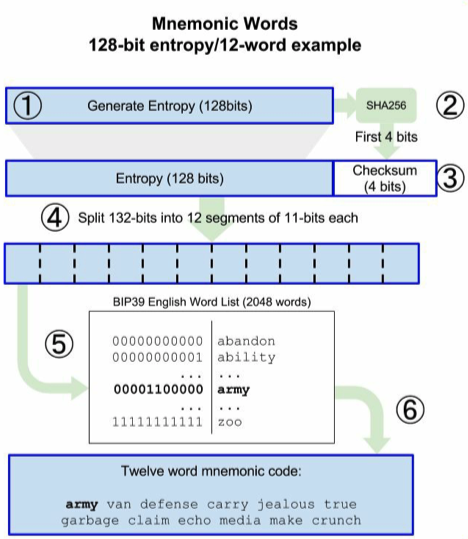
\includegraphics[width=.5\textwidth]{./entropy2mnemonic.png}
\caption{从熵值生成助记词}\label{fig-entropy2mnemonic}
\end{figure}

%下面的列表展示了初始熵值长度ENT,校验和长度与生成的mnemonic sentence长度之间的关系:
%		$$CS = ENT / 32$$
%		$$MS = (ENT + CS) / 11$$
%\begin{table}[h]
%\centering
%\begin{tabular}{|c|c|c|c|c|}
%\hline
%\small
%ENT &  CS  &   ENT+CS  &  MS  \\\hline
%128 &  4  &  132 &  12  \\\hline
%160 &  5  &  165 &  15 \\\hline
%192 &  6  &  198 &  18 \\\hline
%224  &  7  &  231 &  21 \\\hline
%256  &  8  &  264 &  24 \\\hline
%\end{tabular}
%\end{table}

BIP39规定使用\textsf{PBKDF2}函数从助记词生成种子, \textsf{PBKDF2}各参数设置如下:
助记词以UTF-8 NFKD (UTF-8 using Normalization Form Compatibility Decomposition)编码后作为$P$,
``mnemonic''级联$P$同样使用UTF-8 NFKD进行编码后作为盐值$S$,
$c=2048,\ PRF=\textsf{HMAC-SHA512},\ dklen=512$.
最终该算法输出的512比特作为分层确定性钱包的种子.
Listing~\ref{lst-seed}~中的代码基于Trezor的python-mnemonic库\footnote{
\url{https://github.com/trezor/python-mnemonic}}:

\begin{lstlisting}[language=python, caption=基于助记词句子的种子派生, label=lst-seed]
def seed_derivation_from_mnemonic():
    import binascii
    import sys
    from bip32utils import BIP32Key
    if len(sys.argv) > 1:
        data = sys.argv[1]
    else:
        data = sys.stdin.readline().strip()
    data = binascii.unhexlify(data)
    m = Mnemonic('english')
    code=m.to_mnemonic(data)
    seed=m.to_seed(code,'TREZOR')
    xprv = BIP32Key.fromEntropy(seed).ExtendedKey()
    print('mnemonic : %s (%d words)' % (code, len(code.split(' '))))
    print('seed     : %s (%d bits)' % (binascii.hexlify(seed),len(seed) * 4))
    print('xprv     : %s' % xprv)
\end{lstlisting}

\begin{lstlisting}[language=bash, caption = Listing~\ref{lst-seed}~的执行结果示例]
mnemonic : void come effort suffer camp survey warrior heavy shoot primary clutch crush open amazing screen patrol group space point ten exist slush involve unfold (24 words) 

seed : 01f5bced59dec48e362f2c45b5de68b9fd6c92c6634f44d6d40aab69056506f0e35524a    518034ddc1192e1dacd32c1ed3eaa3c3b131c88ed8e7e54c49a5d0998 (256 bits) 

xprv : xprv9s21ZrQH143K39rnQJknpH1WEPFJrzmAqqasiDcVrNuk926oizzJDDQkdiTv
       NPr2FYDYzWgiMiC63YmfPAa2oPyNB23r2g7d1yiK6WpqaQS
\end{lstlisting}